\documentclass[11pt]{charter}

% El títulos de la memoria, se usa en la carátula y se puede usar el cualquier lugar del documento con el comando \ttitle
\titulo{Sistema de control de granja } 

% Nombre del posgrado, se usa en la carátula y se puede usar el cualquier lugar del documento con el comando \degreename
%\posgrado{Carrera de Especialización en Sistemas Embebidos}
%\posgrado{Carrera de Especialización en Internet de las Cosas} 
%\posgrado{Carrera de Especialización en Intelegencia Artificial}
%\posgrado{Maestría en Sistemas Embebidos} 
\posgrado{Maestría en Internet de las cosas}

% Tu nombre, se puede usar el cualquier lugar del documento con el comando \authorname
\autor{Katherine E. Aguirre M.} 

% El nombre del director y co-director, se puede usar el cualquier lugar del documento con el comando \supname y \cosupname y \pertesupname y \pertecosupname
\director{William de J. Mercado M.}
\pertenenciaDirector{UNEG} 
% FIXME:NO IMPLEMENTADO EL CODIRECTOR ni su pertenencia
%\codirector{} % si queda vacio no se deberíá incluir 
%\pertenenciaCoDirector{}

% Nombre del cliente, quien va a aprobar los resultados del proyecto, se puede usar con el comando \clientename y \empclientename
%\cliente{}
%\empresaCliente{}

% Nombre y pertenencia de los jurados, se pueden usar el cualquier lugar del documento con el comando \jurunoname, \jurdosname y \jurtresname y \perteunoname, \pertedosname y \pertetresname.
\juradoUno{Nombre y Apellido (1)}
\pertenenciaJurUno{pertenencia (1)} 
\juradoDos{Nombre y Apellido (2)}
\pertenenciaJurDos{pertenencia (2)}
\juradoTres{Nombre y Apellido (3)}
\pertenenciaJurTres{pertenencia (3)}
 
\fechaINICIO{24 de agosto de 2020}		%Fecha de inicio de la cursada de GdP \fechaInicióname
\fechaFINALPlanificación{22 de Agosto de 2021} 	%Fecha de final de cursada de GdP
\fechaFINALTrabajo{22 de diciembre de 2021}		%Fecha de defensa pública del trabajo final


\begin{document}

\maketitle
\thispagestyle{empty}
\pagebreak


\thispagestyle{empty}
{\setlength{\parskip}{0pt}
\tableofcontents{}
}
\pagebreak


\section{Registros de cambios}
\label{sec:registro}


\begin{table}[ht]
\label{tab:registro}
\centering
\begin{tabularx}{\linewidth}{@{}|c|X|c|@{}}
\hline
\rowcolor[HTML]{C0C0C0} 
Revisión & \multicolumn{1}{c|}{\cellcolor[HTML]{C0C0C0}Detalles de los cambios realizados} & Fecha      \\ \hline
1.0      & Creación del documento                                          & 26/08/2020 \\ \hline
1.1      & Actualización de los primeros 6 temas                           & 04/09/2020 \\ \hline
%\1.2      & Otro ejemplo \newline
%\		   Con texto partido \newline
%\		   En varias líneas \newline
%\		   A propósito                                                     & dd/mm/aaaa \\ \hline
\end{tabularx}
\end{table}

\pagebreak

%-------------------------------------------------------
\section{Acta de constitución del proyecto}
\label{sec:acta}

\begin{flushright}
Buenos Aires, \fechaInicióname
\end{flushright}

\vspace{2cm}

Por medio de la presente se acuerda con la Ing. \authorname\hspace{1px} que su Trabajo Final de la \degreename\hspace{1px} se titulará ``\ttitle'', consistirá esencialmente en el diseño de un Sistema de Monitoreo y Control de Variables Medioambientales en una Granja, y tendrá un presupuesto preliminar estimado de 600 hs de trabajo  y \textcolor{red}{\$XXX}, con fecha de inicio \fechaInicióname\hspace{1px} y fecha de presentación pública \fechaFinalName.

Se adjunta a esta acta la planificación inicial.

\vfill

% Esta parte se construye sola con la información que hayan cargado en el preámbulo del documento y no debe modificarla
\begin{table}[ht]
\centering
\begin{tabular}{ccc}
\begin{tabular}[c]{@{}c@{}}Ariel Lutenberg \\ Director posgrado FIUBA\end{tabular} & \hspace{2cm} %& 
%\begin{tabular}[c]{@{}c@{}}\clientename \\ \empclientename \end{tabular} 
\vspace{2.5cm} \\ 
\multicolumn{3}{c}{\begin{tabular}[c]{@{}c@{}} \supname \\ Director del Trabajo Final\end{tabular}} \vspace{2.5cm} \\
%\begin{tabular}[c]{@{}c@{}}\jurunoname \\ Jurado del Trabajo Final\end{tabular}     &  & \begin{tabular}[c]{@{}c@{}}\jurdosname\\ Jurado del Trabajo Final\end{tabular}  \vspace{2.5cm}  \\
%\multicolumn{3}{c}{\begin{tabular}[c]{@{}c@{}} \jurtresname\\ Jurado del Trabajo Final\end{tabular}} \vspace{.5cm}                                                                     
\end{tabular}
\end{table}
%-------------------------------------------------------
\section{Descripción técnica-conceptual del proyecto a realizar}
\label{sec:descripción}

\begin{consigna}{black} 
Referenciando al prototipo conceptual del Sistema de Control Granja se crea la necesidad de diseñar y desarrollar un sistema acorde a los requerimientos actuales de tecnología, comunicaciones y seguridad que se adecuen al criterio de Internet de las Cosas manejado hoy día, de esta manera se origina un proyecto basado en la premisa de automatizar tareas de monitoreo continuo de temperatura, humedad, calidad del aire, flujo de agua y activación de sistemas de acondicionamiento ambiental de las naves de las granjas de producción animal bajo condiciones controladas, garantizando así el poder adecuarlas a los valores de bienestar ideal que optimizan la crianza de animales y productos relacionados para el consumo humano. 

El planteamiento parte del \textit{knowhow} obtenido en el desarrollo del prototipo conceptual del Sistema de Control Granja, entendiendo el ¿por qué? de las fallas encontradas tanto de seguridad como de latencia, comunicaciones, diseño entre otros, aplicando las buenas practicas que rigen para el desarrollo de este tipo de soluciones y generar de esta manera un producto robusto que reduzca al minimo probable dichas falencias y converja al maximo posible entre la eficiencia y la eficacia.

Del mismo modo, en la Figura \ref{fig:diagBloques} se puede observar el diagrama de bloques que corformará el nuevo sistema, el cual contara con los siguientes modulos: 
\begin{enumerate}
\item Sensores y Actuadores: conjunto de dispositivos cuya finalidad es la de capturar la telemetria o ejecutar ciertas acciones, contaran con un portal cautivo.
\begin{itemize}
\item Portal Cautivo: sistema de administración de los sensores.
\end{itemize}
\item Broker MQTT: servicio que se encargará de recepcionar los mensajes enviados por los clientes y distribuirlos entre sí en el sistema pub-sub.
\item Servicio NTP: Permitirá sincronizar los relojes de los sensores con el servidor.
\item Api - WebService: servicio que permitirá el intercambio de datos entre las aplicaciones.
\item Motor de Base de Datos: repositorio para almacenamiento y persistencia de los datos.
\item Aplicaciones: software para interactuar con los distintos bloques que integran el sistema, a saber:
	\begin{itemize}
		\item App Web: sistema alojado en el servidor que podra ser accedido via wrobser.
		\item App Mobile: sistema para dispositivos móviles.
		\item Sistema de Mensajería y Alertas: Sistema de soporte para el manejo de eventualidades, reportes o alertas.
	\end{itemize}
\end{enumerate}

%-------------------------------------------------------

\vspace{25px}

\begin{figure}[htpb]
\centering 
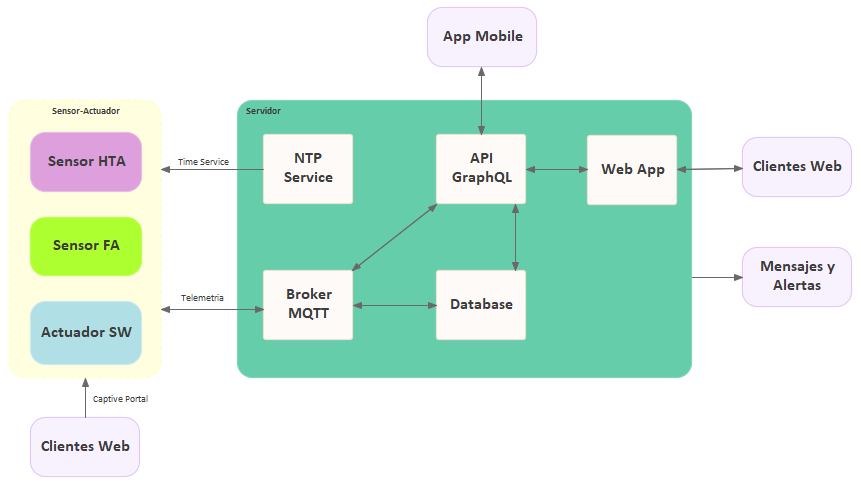
\includegraphics[width=.7\textwidth]{./Figuras/diagBloquesSCG.png}
\caption{Diagrama en bloques del sistema}
\label{fig:diagBloques}
\end{figure}

\vspace{25px}
\end{consigna}


\section{Identificación y análisis de los interesados}
\label{sec:interesados}

\begin{consigna}{red} 

%Nota: (borrar esto y todas las consignas en color rojo antes de entregar este documento).
% 
%Es inusual que una misma persona esté en más de un rol, incluso en proyectos chicos.
% 
%Si se considera que una persona cumple dos o más roles, entonces sólo dejarla en el rol más importante. Por ejemplo:
%
%\begin{itemize}
%\item Si una persona es Cliente pero también colabora u orienta, dejarla solo como Cliente.
%\item Si una persona es el Responsable, no debe ser colocado también como Miembro del equipo.
%\end{itemize}
%
%Pero en cambio sí es usual que el Cliente y el Auspiciante sean el mismo, por ejemplo.


\begin{table}[ht]
%\caption{Identificación de los interesados}
%\label{tab:interesados}
\begin{tabularx}{\linewidth}{@{}|l|X|X|l|@{}}
\hline
\rowcolor[HTML]{C0C0C0} 
Rol           & Nombre y Apellido & Organización 	& Puesto 	\\ \hline
%Auspiciante   & -                 & -           	& -     	\\ \hline
%Cliente       & -                 & -            	& -     	\\ \hline
%Impulsor      & -                 & -            	& -      	\\ \hline
Responsable   & \authorname       & FIUBA        	& Alumno 	\\ \hline
%Colaboradores & -                 & -            	& -      	\\ \hline
Orientador    & \supname	      & \pertesupname 	& Director	Trabajo final \\ \hline
%Equipo        & - & -	& -   	\\ \hline
%Opositores    & -                 & -            	& -      	\\ \hline
%Usuario final & -                 & -            	& -      	\\ \hline
\end{tabularx}
\end{table}

%El Director suele ser uno de los Orientadores.
%
%No dejar celdas vacías; si no hay nada que poner en una celda colocar un signo ``-''.
%
%No dejar filas vacías; si no hay nada que poner en una fila entonces eliminarla.
%
%Sería deseable listar a continuación de la tabla las principales características de cada interesado.
% 
%Por ejemplo:
%\begin{itemize}
%\item Auspiciante: es riguroso y exigente con la rendición de gastos. Tener mucho cuidado con esto.
%\item Equipo: Juan Perez, suele pedir licencia porque tiene un familiar con una enfermedad. Planificar considerando esto.
%\item Orientador: María Gómez, nos va a poder ayudar mucho con la gestión de impuestos.
%\end{itemize}

\end{consigna}

%-------------------------------------------------------
\section{1. Propósito del proyecto}
\label{sec:proposito}
\begin{consigna}{black} 
El propósito de este proyecto es el de diseñar y producir un Sistema para Monitoreo y Control de Variables Medioambientales aplicado a Granjas de producción animal, aplicando las buenas practicas que rigen en el desarrollo de soluciones IoT de manera óptima, tomando como referencia un prototipo conceptual basado en granja avícola.
\end{consigna}

%-------------------------------------------------------
\section{2. Alcance del proyecto}
\label{sec:alcance}

\begin{consigna}{black}
%¿Qué se incluye y que no se incluye en este proyecto?
%
%Se refiere al trabajo a hacer para entregar el producto o resultado especificado. 
%
%Explicitar todo lo quede comprendido dentro del alcance del proyecto.
%
%Explicitar además todo lo que no quede incluido (``El presente proyecto no incluye...'')
El alcance del proyecto contempla el desarrollo e implementación de los distintos modulos que componen el sistema en su totalidad y las tareas complemantarias que ayudaran a alcanzar los objetivos planteados, a saber:

\begin{enumerate}
	\item \textbf{Realizar capacitaciones y entrenamientos necesarios para completar los desarrollos en las teconologías seleccionadas}: es mandatorio realizar capacitaciones en diversas teconologías de desarrollo de software para poder completar las tareas, se necesita entrenamiento en: GraphQL y React Native.
	\item \textbf{Configuración del servidor}: se contempla la instalación y configuración de Raspbian Buster lite para plataforma X86 en una Raspberry Pi, así como la generación de certificados para la configuración de las conexiones seguras.	
	\item \textbf{Diseño e implementación de la Base de Datos}: se debe definir el esquema y diagramas de la base datos, realizar la codificación y construcción de la misma en el motor de base de datos seleccionado.
	\item \textbf{Implementación del servicio NTP}: se deben realizar las instalaciones y configuraciones necesarias para poner en funciónamiento el servicio de \textit{Network Time Protocol}.
	\item \textbf{Implementación del Broker MQTT}: se necesita instalar, configurar y securizar el servidor MQTT así como configurar la conexión con la base de datos para persistir la telemetria.
	\item \textbf{Diseño, desarrollo e instalación del software en los sensores}: se necesita desarrollar el sistema de administración de los sensores así como la implementación de los protocolos de comunicación y seguridad necesarios para el envío y recepción de telemetría.
	\item \textbf{Diseño, desarrollo e implementación de la API-WebService}: se debe desarrollar e implementar el WebService que permitirá interactuar a los diferentes clientes con el resto de los modulos habilitados para ello.
	\item \textbf{Diseño, desarrollo e implementación de la App Hibrida}: desarrollar e instalar, según la tecnología, las aplicaciones web y moviles que interactuaran con el WebService.
	\item \textbf{Pruebas Generales del sistema}: cada uno de los modulos que compone el sistema debera ser testeado para asegurar la calidad y funcionamiento de los mismos.
	\item \textbf{Elaboración de los manuales de configuración e instalación de cada modulo}: es mandatorio elaborar los manuales de instalación, configuración y/o uso de cada modulo desarrollado.
\end{enumerate}
\end{consigna}

%-------------------------------------------------------
\section{3. Supuestos del proyecto}
\label{sec:supuestos}

\begin{consigna}{black}
Para el desarrollo del presente proyecto se supone que: 

\begin{itemize}
	\item El hardware de los sensores y actuadores ya está elaborado por lo que el desarrollo de los mismos se limita al desarrollo e instalación del software, igualmente se cuenta con el hardware y software necesario para configurar el servidor y las estaciones de desarrollo donde será construido  el proyecto.
	\item Se determinó satisfactoriamente la factibilidad técnica del desarrollo de los distintos elementos que componen el proyecto.
	\item Se determinó que existe la disponibilidad de tiempo para recibir capacitación, diseñar, desarrollar e implementar todo el proyecto.
	\item Respecto a las reglamentaciones y leyes existentes se determinó que no existe impedimento alguno para culminar exitosamente el proyecto.
	\item Respecto a la situación presupuestaria del equipo de desarrollo se determinó que no existe impedimento alguno para subsanar los gastos e enversiones necesarias para completar el proyecto.
\end{itemize}
%
%Por ejemplo, se podrían incluir supuestos respecto a disponibilidad de tiempo y recursos humanos y materiales, sobre la factibilidad técnica de distintos aspectos del proyecto, sobre otras cuestiones que sean necesarias para el éxito del proyecto como condiciones macroeconómicas o reglamentarias.
\end{consigna}

%-------------------------------------------------------

\section{4. Requerimientos}
\label{sec:requerimientos}
\begin{consigna}{black}
Los requerimientos necesarios para el desarrollo del proyecto son los siguientes:
\begin{enumerate}
\item Grupo de requerimientos asociados con sensores y actuadores:
	\begin{enumerate}
		\item Deberá activarse en modo servidor cuando no esté conectado a una SSID externa y de esta manera activar el portal de configuración del mismo en un servidor local, una vez conectado a la WiFI externa se deshabilitará la WiFi interna (ésta sólo estará activa en casos de desconección con la WiFI externa) y fungirá como servidor web donde podrá ser consultada su funcionalidad y telemetría.
		\item Dentro de los servicios a manejar o configurar en el dispositivo se tienen: MQTT (Suscripción y Publicación de tópicos), NTP, Acceso a la telemetría, Administración de Redes Wifi tanto interna como externa, Administración de usuario y contraseña, Reset valores de fábrica, Reinicio del dispositivo, Test de hardware.
		\item Se contempla la actualización remota de los dispositivos habilitando la opción Update OTA en los mismos.
		\item Se requiere que las comunicaciones se realicen en formato JSON.
		\item Deberá ser capaz de publicar datos de su funcionamiento para que sean registrados y procesados posteriormente según sea la necesidad, estas comunicaciones deberán estar encriptadas mediante el uso de comunicaciones seguras con SSL/TLS, usuario y contraseña para garantizar la privacidad en el transporte de datos.
		\item Deberá poder conectarse a un servidor NTP para tener su hora sincronizada y así poder manejar cabeceras de tiempo en los registros enviados en formato JSON.
	\end{enumerate}
\item Grupo de requerimientos asociados con el servicio NTP:
	\begin{enumerate}
		\item Se debera contar con un servicio de hora que pueda funcionar offline en caso de fallar la conectividad a internet para así poder sincronizar las operaciones.
	\end{enumerate}
\item Grupo de requerimientos asociados con la Base de Datos:
	\begin{enumerate}
		\item Se requiere la instalación y configuración del motor de base de datos para su posterior uso, el cual deberá ser Postgres o MongoDB en su defecto.
		\item Se requiere diseñar y elaborar el esquema de la base de datos según los siguientes puntos:
			\begin{enumerate}
				\item Usuarios
				\item Roles
				\item Alarmas, mensajes y escalas de severidades.
				\item Permisos
				\item Estados
				\item Zonas de acción
				\item Lecturas de datos
				\item Telemetría
				\item Dispositivos
				\item Tipos bases
			\end{enumerate}
		\item Se requiere que los datos puedan ser registrados en formato JSON.
	\end{enumerate}
\item Grupo de requerimientos asociados con el Broker MQTT:
	\begin{enumerate}
		\item Se requiere la instalación y configuración de mosquitto como gestor de Pub-Sub.
		\item Publicación: telemetría, estatus del dispositivo, poder de la señal wifi, versión del firmware.
		\item Suscripción: activación o desactivación de actuadores de forma manual según el tiempo definido, requerir datos específicos por ítem de los mencionados en el punto previo.
		\item Registro de datos en la Base de Datos.
		\item Se requiere que las comunicaciones se realicen en formato JSON.
	\end{enumerate}	
\item Grupo de requerimientos asociados con Api - WebService:
	\begin{enumerate}
		\item En un principio se plantea la posibilidad de desarrollar la Api en GraphQL con Node.js, sino es factible se empleará Spring Boot 2 sobre Apache Tomcat.
		\item Deberá manejar inicios de sesión autenticados así como comunicaciones seguras tanto con el Broker como con los clientes y la base de datos.
		\item Se contempla que la API sea capaz de enviar alertas de alarmas vía email, tweets, chats de telegram o mensajes IFTTT.
		\item Se requiere que las comunicaciones se realicen en formato JSON.
		\item Dentro de los endpoints a definir se encuentran los siguientes gestiones:
		\begin{itemize}
		\item Usuarios.
		\item Roles de usuarios.
		\item Configuraciones varias
		\item Tipos: alarmas, sensores
		\item Zonas a monitorear.
		\item Permisos.
		\item Estados.
		\item Sensores.
		\item Lecturas de Datos
		\item Alarmas Generadas
		\item Escala de Severidades de alarmas
		\item Categorías de Clasificación de registros
		\item Consulta de telemetría por sensor.
		\item Activación de actuadores.
		\item MQTT: Suscripción y Publicación de tópicos
		\item NTP
		\end{itemize}
	\end{enumerate}	
\item Grupo de requerimientos asociados con la App:
	\begin{enumerate}
		\item El cliente será una App basada en JS, se plantea la posibilidad de hacerla multiplataforma con soporte para dispositivos mobile (Android, IOS) y para navegadores (Chrome, Firefox, Safari) tanto de escritorios (Windows, MacOS, Linux) como tablets (Android, Ipad). 
		\item Se requiere SSL/Tls en todas las comunicaciones.
		\item Se recomienda el uso de React Native.
		\item Se requiere que las comunicaciones se realicen en formato JSON.
	\end{enumerate}		
\end{enumerate}
%
%Leyendo los requerimientos se debe poder interpretar cómo será el proyecto y su funciónalidad.
%
%De ser posible indicar cómo se obtuvieron cada uno de los requerimientos 
%
%Indicar claramente cuál es la prioridad entre los distintos requerimientos. 
%
%No olvidarse de que los requerimientos incluyen a las regulaciones y normas vigentes!!!
%
%Y al escribirlos seguir las siguientes reglas:
%\begin{itemize}
%\item Ser breve y conciso (nadie lee cosas largas). 
%\item Ser específico: no dejar lugar a confusiones.
%\item Expresar los requerimientos en términos que sean cuantificables y medibles.
%\end{itemize}
\end{consigna}

\section{Historias de usuarios (\textit{Product backlog})}
\label{sec:backlog}

\begin{consigna}{black}
Descripción: En esta sección se deben incluir las historias de usuarios y su ponderación (\textit{history points}). Recordar que las historias de usuarios son descripciones cortas y simples de una característica contada desde la perspectiva de la persona que desea la nueva capacidad, generalmente un usuario o cliente del sistema. La ponderación es un número entero que representa el tamaño de la historia comparada con otras historias de similar tipo.
\end{consigna}

\section{5. Entregables principales del proyecto}
\label{sec:entregables}

\begin{consigna}{black}
Se contemplan los siguientes entregables en el transcurso del proyecto hasta su finalización: 
	\begin{itemize}
		\item Manual de uso de las aplicaciones y sistemas cautivos.
		\item Diagrama esquemático general del sistema y de la base de datos
		\item Código fuente de sistema cautivo, API WebService, aplicaciones, backup de la  base de datos.
		\item Manual de instalación de las aplicaciones mobiles, portales cautivos, base de datos, broker, API WebService y servidor NTP.
		\item Informe final.
	\end{itemize}
\end{consigna}

\section{6. Desglose del trabajo en tareas}
\label{sec:wbs}

\begin{consigna}{black}
Se recomienda mostrar el WBS mediante una lista indexada:

\begin{enumerate}
\item Capacitaciones y Entrenamientos
	\begin{enumerate}
		\item Entrenamiento en GraphQL. (14 hrs)
		\item Entrenamiento en React Native. (20 hrs)
	\end{enumerate}
\item Configuración del Servidor
	\begin{enumerate}
		\item Instalación del OS. (2 hr)
		\item Ajuste de Configuraciones. (1 hrs)
		\item Generación y seteo de certificados seguros. (1 hrs)
		\item Instalación de aplicaciones administrativas del server:
		\begin{itemize}
			\item WebMin. (0.5 hrs)
			\item Docker. (0.25 hrs)
			\begin{itemize}
				\item Mosquitto. (0.25 hrs) 
				\item NTP. (0.25 hrs)
			\end{itemize}
		\end{itemize}
		\item Elaboración del manual de instalación. (1 hrs)
	\end{enumerate}
\item Base de Datos
	\begin{enumerate}
		\item Instalación de Postgres - MongoDB. (0.5 hrs)
		\item Puesta a punto de la Base de Datos. (1 hrs)
		\item Diseño y desarrollo del esquema de la BD. (12 hrs)
		\item Elaboración del manual de instalación y configuración. (4 hrs)
	\end{enumerate}
\item Servicio NTP 
	\begin{enumerate}
		\item Configuración del servicio. (0.25 hrs)
		\item Pruebas de Funcionamiento. (0.5 hrs)
		\item Elaboración del manual de instalación y configuración. (0.25 hrs)
	\end{enumerate}
\item Broker MQTT
	\begin{enumerate}
		\item Configuración del servicio. (1 hrs)
		\item Pruebas de Funcionamiento. (0.5 hrs)
		\item Elaboración del manual de instalación y configuración. (2 hrs)
	\end{enumerate}
\item Sensores y Actuadores
	\begin{enumerate}
		\item Desarrollo del software de control:
		\begin{itemize}
			\item Gestion de memoria no volatil y configuraciones (6 hrs)
			\item Sección NTP. (6 hrs)
			\item Sección MQTT. (12 hrs)
			\item Implementación de OTA. (12 hrs)
		\end{itemize}
		\item Desarrollo del portal cautivo:
		\begin{itemize}
			\item Gestión de NTP. (3 hrs)
			\item Gestión de MQTT. (3 hrs)
			\item Gestión de Usuario. (3 hrs)
			\item Gestión de SSID Externa. (3 hrs)
			\item Gestión de SSID Interna. (3 hrs)
			\item Reseteo y Reinicio. (3 hrs)
			\item Informe de test de hardware. (6 hrs)
		\end{itemize}
		\item Pruebas de Funcionamiento. (3 hrs)
		\item Elaboración del manual de instalación y configuración. (6 hrs)
	\end{enumerate}
\item Api Webservice
	\begin{enumerate}
		\item Configuración del Entorno de Desarrollo. (2 hrs)
		\item Desarrollo de Endpoints (CRUD):
		\begin{itemize}
			\item Sesiones seguras. (12 hrs)
			\item Usuarios:
			\begin{itemize}
				\item Gestión de ``Mi Espacio``:
				\begin{itemize}
					\item Datos personales: Nombre, dirección, celulares, correos, twitter, foto. (6 hrs)
				\end{itemize}
				\item Administración de:
				\begin{itemize}
					\item Altas y bajas. (6 hrs) 
					\item Roles. (3 hrs)
					\item Zonas. (3 hrs)
					\item Permisos. (3 hrs)
				\end{itemize}
			\end{itemize}
			\item Tipos: alarmas, notificaciones y sensores. (12 hrs) 
			\item Zonas a monitorear. (6 hrs) 
			\item Permisos. (6 hrs) 
			\item Estados. (6 hrs) 
			\item Sensores. (6 hrs) 
			\item Gestión de Datos:
			\begin{itemize}
				\item Lectura de datos: por sensores y zonas. (18 hrs) 
				\item visualización de reportes: por rango de fechas, horas y zonas. (24 hrs) 
			\end{itemize}
			\item Alarmas y notificaciones. (6 hrs) 
			\item Severidades. (6 hrs) 
			\item MQTT: Suscripción y publicación de tópicos. (12 hrs) 
			\item Gestión de Categorías de Clasificación. (6 hrs) 
			\item Configuraciones varias del entorno: servidor sendmail, telegram, IFTTT. (12 hrs) 
			\item Elaboración del manual de instalación y configuración. (36 hrs)  
		\end{itemize}
	\end{enumerate}
\item Aplicaciones
	\begin{enumerate}
		\item Configuración del Entorno de Desarrollo. (2 hrs) 
		\item Desarrollo de Endpoints (CRUD):
		\begin{itemize}
			\item Usuarios:
			\begin{itemize}
				\item Sesiones. (12 hrs) 
				\item Gestión de ``Mi Espacio``:
				\begin{itemize}
					\item Datos personales: Nombre, dirección, celulares, correos, twitter, foto. (24 hrs) 
				\end{itemize}
				\item Administración de:
				\begin{itemize}
					\item Altas y bajas. (6 hrs) 
					\item Roles. (3 hrs) 
					\item Zonas. (3 hrs) 
					\item Permisos. (3 hrs) 
				\end{itemize}
			\end{itemize}
			\item Tipos: alarmas, notificaciones y sensores. (6 hrs) 
			\item Zonas a monitorear. (6 hrs) 
			\item Permisos. (6 hrs) 
			\item Estados. (6 hrs) 
			\item Sensores. (6 hrs) 
			\item Gestión de Datos:
			\begin{itemize}
				\item Lectura de datos: por sensores y zonas. (18 hrs) 
				\item visualización de reportes: por rango de fechas, horas y zonas. (24 hrs) 
			\end{itemize}
			\item Alarmas y notificaciones. (6 hrs) 
			\item Severidades. (6 hrs) 
			\item MQTT: Suscripción y publicación de topicos. (12 hrs) 
			\item Gestión de Categorías de Clasificación. (6 hrs) 
			\item Configuraciones varias del entorno: servidor sendmail, telegram, IFTTT. (12 hrs)
			\item Pruebas de Funciónamiento
			\item Elaboración del manual de instalación y configuración
		\end{itemize}
	\end{enumerate}	
\item Informe Final
	\begin{itemize}
		\item Redacción del Informe Final. (63 hrs)
	\end{itemize}
\end{enumerate}

%Cantidad total de horas: (tantas hs)
%
%Se recomienda que no haya ninguna tarea que lleve más de 40 hs. 

\end{consigna}

\section{7. Diagrama de Activity On Node}
\label{sec:AoN}

\begin{consigna}{red}
Armar el AoN a partir del WBS definido en la etapa anterior. 

%La figura \ref{fig:AoN} fue elaborada con el paquete latex tikz y pueden consultar la siguiente referencia \textit{online}:

%\url{https://www.overleaf.com/learn/latex/LaTeX_Graphics_using_TikZ:_A_Tutorial_for_Beginners_(Part_3)\%E2\%80\%94Creating_Flowcharts}

\end{consigna}

\begin{figure}[htpb]
\centering 
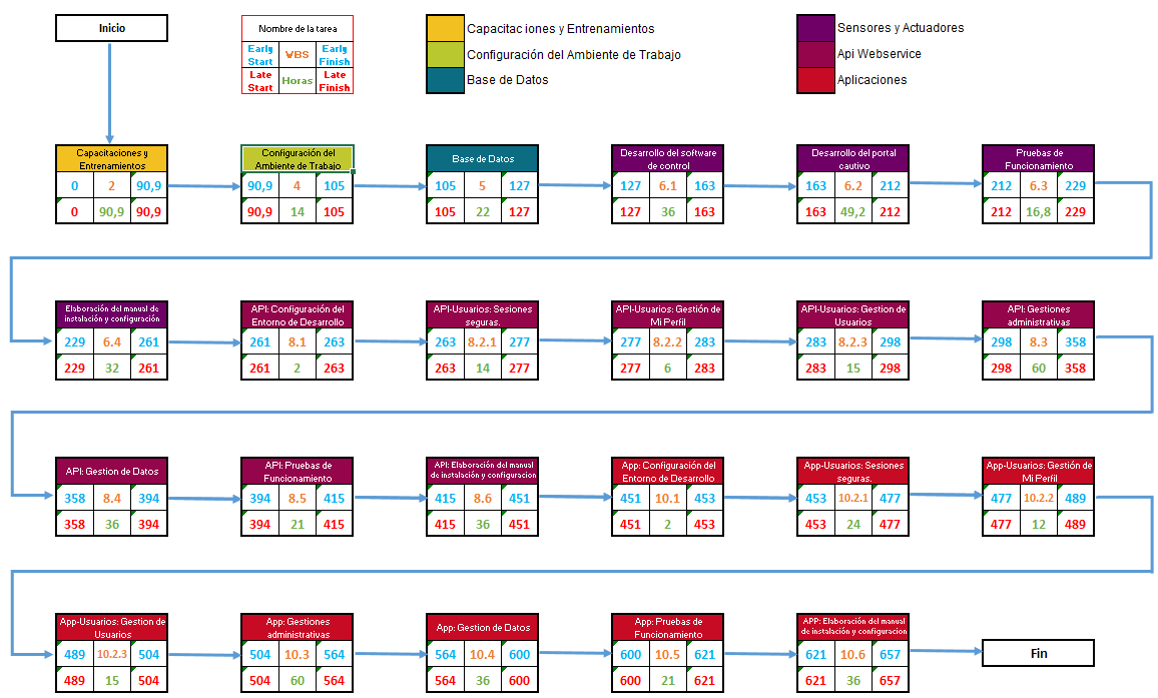
\includegraphics[width=.8\textwidth]{./Figuras/AoN.png}
\caption{Diagrama en \textit{Activity on Node}}
\label{fig:AoN}
\end{figure}

Indicar claramente en qué unidades están expresados los tiempos.
De ser necesario indicar los caminos semicríticos y analizar sus tiempos mediante un cuadro.
Es recomendable usar colores y un cuadro indicativo describiendo qué representa cada color, como se muestra en el siguiente ejemplo:



\section{8. Diagrama de Gantt}
\label{sec:gantt}

\begin{consigna}{red}
Utilizar el software Gantter for Google Drive o alguno similar para dibujar el diagrama de Gantt.

Existen muchos programas y recursos \textit{online} para hacer diagramas de gantt, entre las cuales destacamos:

\begin{itemize}
\item Planner
\item GanttProject
\item Trello + \textit{plugins}. En el siguiente link hay un tutorial oficial: \\ \url{https://blog.trello.com/es/diagrama-de-gantt-de-un-proyecto}
\item Creately, herramienta online colaborativa. \\\url{https://creately.com/diagram/example/ieb3p3ml/LaTeX}
\item Se puede hacer en latex con el paquete \textit{pgfgantt}\\ \url{http://ctan.dcc.uchile.cl/graphics/pgf/contrib/pgfgantt/pgfgantt.pdf}
\end{itemize}

Pegar acá una captura de pantalla del diagrama de Gantt, cuidando que la letra sea suficientemente grande como para ser legible. 
Si el diagrama queda demasiado ancho, se puede pegar primero la ``tabla'' del Gantt y luego pegar la parte del diagrama de barras del diagrama de Gantt.

Configurar el software para que en la parte de la tabla muestre los códigos del EDT (WBS).\\
Configurar el software para que al lado de cada barra muestre el nombre de cada tarea.\\
Revisar que la fecha de finalización coincida con lo indicado en el Acta Constitutiva.

En la figura \ref{fig:gantt}, se muestra un ejemplo de diagrama de gantt realizado con el paquete de \textit{pgfgantt}. En la plantilla pueden ver el código que lo genera y usarlo de base para construir el propio.

\begin{figure}[htbp]
\begin{center}
\begin{ganttchart}{1}{12}
  \gantttitle{2020}{12} \\
  \gantttitlelist{1,...,12}{1} \\
  \ganttgroup{Group 1}{1}{7} \\
  \ganttbar{Task 1}{1}{2} \\
  \ganttlinkedbar{Task 2}{3}{7} \ganttnewline
  \ganttmilestone{Milestone o hito}{7} \ganttnewline
  \ganttbar{Final Task}{8}{12}
  \ganttlink{elem2}{elem3}
  \ganttlink{elem3}{elem4}
\end{ganttchart}
\end{center}
\caption{Diagrama de gantt de ejemplo}
\label{fig:gantt}
\end{figure}

\end{consigna}

\section{9. Matriz de uso de recursos de materiales}
\label{sec:recursos}


\begin{table}
\label{tab:recursos}
\centering
\begin{tabularx}{\linewidth}{@{}|c|X|X|X|X|c|@{}}
\hline
\cellcolor[HTML]{C0C0C0} & \cellcolor[HTML]{C0C0C0} & \multicolumn{4}{c|}{\cellcolor[HTML]{C0C0C0}Recursos requeridos (horas)} \\ \cline{3-6} 
\multirow{-2}{*}{\cellcolor[HTML]{C0C0C0}\begin{tabular}[c]{@{}c@{}}Código\\ WBS\end{tabular}} & \multirow{-2}{*}{\cellcolor[HTML]{C0C0C0}\begin{tabular}[c]{@{}c@{}}Nombre \\ tarea\end{tabular}} & Material 1 & Material 2 & Material 3 & Material 4 \\ \hline
 &  &  &  &  &  \\ \hline
 &  &  &  &  &  \\ \hline
 &  &  &  &  &  \\ \hline
 &  &  &  &  &  \\ \hline
 &  &  &  &  &  \\ \hline
 &  &  &  &  &  \\ \hline
 &  &  &  &  &  \\ \hline
 &  &  &  &  &  \\ \hline 
 &  &  &  &  &  \\ \hline
 &  &  &  &  &  \\ \hline
 &  &  &  &  &  \\ \hline
 &  &  &  &  &  \\ \hline
 &  &  &  &  &  \\ \hline
 &  &  &  &  &  \\ \hline
 &  &  &  &  &  \\ \hline
 &  &  &  &  &  \\ \hline
 &  &  &  &  &  \\ \hline
 &  &  &  &  &  \\ \hline
 &  &  &  &  &  \\ \hline
 &  &  &  &  &  \\ \hline
 &  &  &  &  &  \\ \hline
 &  &  &  &  &  \\ \hline
 &  &  &  &  &  \\ \hline
 &  &  &  &  &  \\ \hline 
 &  &  &  &  &  \\ \hline
 &  &  &  &  &  \\ \hline
 &  &  &  &  &  \\ \hline
 &  &  &  &  &  \\ \hline

\end{tabularx}%
\end{table}


\section{10. Presupuesto detallado del proyecto}
\label{sec:presupuesto}

\begin{consigna}{red}
Si el proyecto es complejo entonces separarlo en partes:
\begin{itemize}
\item Un total global, indicando el subtotal acumulado por cada una de las áreas.
\item El desglose detallado del subtotal de cada una de las áreas.
\end{itemize}

IMPORTANTE: No olvidarse de considerar los COSTOS INDIRECTOS.

\end{consigna}

\begin{table}[htpb]
\centering
\begin{tabularx}{\linewidth}{@{}|X|c|r|r|@{}}
\hline
\rowcolor[HTML]{C0C0C0} 
\multicolumn{4}{|c|}{\cellcolor[HTML]{C0C0C0}COSTOS DIRECTOS} \\ \hline
\rowcolor[HTML]{C0C0C0} 
Descripción &
  \multicolumn{1}{c|}{\cellcolor[HTML]{C0C0C0}Cantidad} &
  \multicolumn{1}{c|}{\cellcolor[HTML]{C0C0C0}Valor unitario} &
  \multicolumn{1}{c|}{\cellcolor[HTML]{C0C0C0}Valor total} \\ \hline
 &
  \multicolumn{1}{c|}{} &
  \multicolumn{1}{c|}{} &
  \multicolumn{1}{c|}{} \\ \hline
 &
  \multicolumn{1}{c|}{} &
  \multicolumn{1}{c|}{} &
  \multicolumn{1}{c|}{} \\ \hline
\multicolumn{1}{|l|}{} &
   &
   &
   \\ \hline
\multicolumn{1}{|l|}{} &
   &
   &
   \\ \hline
\multicolumn{3}{|c|}{SUBTOTAL} &
  \multicolumn{1}{c|}{} \\ \hline
\rowcolor[HTML]{C0C0C0} 
\multicolumn{4}{|c|}{\cellcolor[HTML]{C0C0C0}COSTOS INDIRECTOS} \\ \hline
\rowcolor[HTML]{C0C0C0} 
Descripción &
  \multicolumn{1}{c|}{\cellcolor[HTML]{C0C0C0}Cantidad} &
  \multicolumn{1}{c|}{\cellcolor[HTML]{C0C0C0}Valor unitario} &
  \multicolumn{1}{c|}{\cellcolor[HTML]{C0C0C0}Valor total} \\ \hline
\multicolumn{1}{|l|}{} &
   &
   &
   \\ \hline
\multicolumn{1}{|l|}{} &
   &
   &
   \\ \hline
\multicolumn{1}{|l|}{} &
   &
   &
   \\ \hline
\multicolumn{3}{|c|}{SUBTOTAL} &
  \multicolumn{1}{c|}{} \\ \hline
\rowcolor[HTML]{C0C0C0}
\multicolumn{3}{|c|}{TOTAL} &
   \\ \hline
\end{tabularx}%
\end{table}


\section{11. Matriz de asignación de responsabilidades}
\label{sec:responsabilidades}
\begin{consigna}{red}
Establecer la matriz de asignación de responsabilidades y el manejo de la autoridad completando la siguiente tabla:

\begin{table}[htpb]
\centering
\resizebox{\textwidth}{!}{%
\begin{tabular}{|c|c|c|c|c|c|}
\hline
\rowcolor[HTML]{C0C0C0} 
\cellcolor[HTML]{C0C0C0} &
  \cellcolor[HTML]{C0C0C0} &
  \multicolumn{4}{c|}{\cellcolor[HTML]{C0C0C0}Listar todos los nombres y roles del proyecto} \\ \cline{3-6} 
\rowcolor[HTML]{C0C0C0} 
\cellcolor[HTML]{C0C0C0} &
  \cellcolor[HTML]{C0C0C0} &
  Responsable &
  Orientador &
  Equipo &
  Cliente \\ \cline{3-6} 
\rowcolor[HTML]{C0C0C0} 
\multirow{-3}{*}{\cellcolor[HTML]{C0C0C0}\begin{tabular}[c]{@{}c@{}}Código\\ WBS\end{tabular}} &
  \multirow{-3}{*}{\cellcolor[HTML]{C0C0C0}Nombre de la tarea} &
  \authorname &
  \supname \\ \hline
%  Nombre de alguien &
%  \clientename \\ \hline
 &  &  &  &  &  \\ \hline
 &  &  &  &  &  \\ \hline
 &  &  &  &  &  \\ \hline
\end{tabular}%
}
\end{table}

{\footnotesize
Referencias:
\begin{itemize}
	\item P = Responsabilidad Primaria
	\item S = Responsabilidad Secundaria
	\item A = Aprobación
	\item I = Informado
	\item C = Consultado
\end{itemize}
} %footnotesize

Una de las columnas debe ser para el Director, ya que se supone que participará en el proyecto.
A su vez se debe cuidar que no queden muchas tareas seguidas sin ``A'' o ``I''.

Importante: es redundante poner ``I/A'' o ``I/C'', porque para aprobarlo o responder consultas primero la persona debe ser informada.

\end{consigna}

\section{12. Gestión de riesgos}
\label{sec:riesgos}

\begin{consigna}{red}
a) Identificación de los riesgos (al menos cinco) y estimación de sus consecuencias:
 
Riesgo 1: detallar el riesgo (riesgo es algo que si ocurre altera los planes previstos)
\begin{itemize}
\item Severidad (S): mientras más severo, más alto es el número (usar números del 1 al 10).\\
Justificar el motivo por el cual se asigna determinado número de severidad (S).
\item Probabilidad de ocurrencia (O): mientras más probable, más alto es el número (usar del 1 al 10).\\
Justificar el motivo por el cual se asigna determinado número de (O). 
\end{itemize}   

Riesgo 2:
\begin{itemize}
\item Severidad (S): 
\item Ocurrencia (O):
\end{itemize}

Riesgo 3:
\begin{itemize}
\item Severidad (S): 
\item Ocurrencia (O):
\end{itemize}


b) Tabla de gestión de riesgos:      (El RPN se calcula como RPN=SxO)

\begin{table}[htpb]
\centering
\begin{tabularx}{\linewidth}{@{}|X|c|c|c|c|c|c|@{}}
\hline
\rowcolor[HTML]{C0C0C0} 
Riesgo & S & O & RPN & S* & O* & RPN* \\ \hline
       &   &   &     &    &    &      \\ \hline
       &   &   &     &    &    &      \\ \hline
       &   &   &     &    &    &      \\ \hline
       &   &   &     &    &    &      \\ \hline
       &   &   &     &    &    &      \\ \hline
\end{tabularx}%
\end{table}

Criterio adoptado: 
Se tomarán medidas de mitigación en los riesgos cuyos números de RPN sean mayores a...

Nota: los valores marcados con (*) en la tabla corresponden luego de haber aplicado la mitigación.

c) Plan de mitigación de los riesgos que originalmente excedían el RPN máximo establecido:
 
Riesgo 1: plan de mitigación (si por el RPN fuera necesario elaborar un plan de mitigación).
  Nueva asignación de S y O, con su respectiva justificación:
  - Severidad (S): mientras más severo, más alto es el número (usar números del 1 al 10).
          Justificar el motivo por el cual se asigna determinado número de severidad (S).
  - Probabilidad de ocurrencia (O): mientras más probable, más alto es el número (usar del 1 al 10).
          Justificar el motivo por el cual se asigna determinado número de (O).

Riesgo 2: plan de mitigación (si por el RPN fuera necesario elaborar un plan de mitigación).
 
Riesgo 3: plan de mitigación (si por el RPN fuera necesario elaborar un plan de mitigación).

\end{consigna}


\section{13. Gestión de la calidad}
\label{sec:calidad}

\begin{consigna}{red}
Para cada uno de los requerimientos del proyecto indique:
\begin{itemize} 
\item Req \#1: copiar acá el requerimiento.

Verificación y validación:

\begin{itemize}
\item Verificación para confirmar si se cumplió con lo requerido antes de mostrar el sistema al cliente. Detallar 
\item Validación con el cliente para confirmar que está de acuerdo en que se cumplió con lo requerido. Detallar  
\end{itemize}

\end{itemize}

Tener en cuenta que en este contexto se pueden mencionar simulaciones, cálculos, revisión de hojas de datos, consulta con expertos, mediciones, etc.

\end{consigna}

\section{14. Comunicación del proyecto}
\label{sec:comunicaciones}

El plan de comunicación del proyecto es el siguiente:

\begin{table}[htpb]
\centering
\begin{tabularx}{\linewidth}{@{}|X|C{2.4cm}|C{3cm}|C{1.8cm}|C{2cm}|C{2.1cm}|@{}}
\hline
\rowcolor[HTML]{C0C0C0} 
\multicolumn{6}{|c|}{\cellcolor[HTML]{C0C0C0}PLAN DE COMUNICACIÓN DEL PROYECTO}           \\ \hline
\rowcolor[HTML]{C0C0C0} 
¿Qué comunicar? & Audiencia & Propósito & Frecuencia & Método de comunicac. & Responsable \\ \hline
                &           &           &            &                      &             \\ \hline
                &           &           &            &                      &             \\ \hline
                &           &           &            &                      &             \\ \hline
                &           &           &            &                      &             \\ \hline
                &           &           &            &                      &             \\ \hline
\end{tabularx}
\end{table}

\section{15. Gestión de compras}
\label{sec:compras}

\begin{consigna}{red}
En caso de tener que comprar elementos o contratar servicios:
a) Explique con qué criterios elegiría a un proveedor.
b) Redacte el Statement of Work correspondiente.
\end{consigna}

\section{16. Seguimiento y control}
\label{sec:seguimiento}

\begin{consigna}{red}
Para cada tarea del proyecto establecer la frecuencia y los indicadores con los se seguirá su avance y quién será el responsable de hacer dicho seguimiento y a quién debe comunicarse la situación (en concordancia con el Plan de Comunicación del proyecto).

El indicador de avance tiene que ser algo medible, mejor incluso si se puede medir en \% de avance. Por ejemplo,se pueden indicar en esta columna cosas como ``cantidad de conexiones ruteadeas'' o ``cantidad de funciones implementadas'', pero no algo genérico y ambiguo como ``\%'', porque el lector no sabe porcentaje de qué cosa.

\end{consigna}

\begin{longtable}{|m{1cm}|m{3.5cm}|m{2.2cm}|m{2cm}|m{3cm}|m{1.5cm}|}
\hline
\rowcolor[HTML]{C0C0C0} 
\multicolumn{6}{|c|}{\cellcolor[HTML]{C0C0C0}SEGUIMIENTO DE AVANCE}                                                                       \\ \hline
\rowcolor[HTML]{C0C0C0} 
Tarea del WBS 			& Indicador de avance & Frecuencia de reporte & Resp. de seguimiento & Persona a ser informada & Método de comunic. \\ \hline
\endfirsthead

\hline
\rowcolor[HTML]{C0C0C0} 
\multicolumn{6}{c}{\cellcolor[HTML]{C0C0C0}SEGUIMIENTO DE AVANCE}                                                                       \\ \hline
\rowcolor[HTML]{C0C0C0} 
Tarea del WBS 			& Indicador de avance & Frecuencia de reporte & Resp. de seguimiento & Persona a ser informada & Método de comunic. \\ \hline
\endhead

\multicolumn{6}{c}{Continúa}
\endfoot

\endlastfoot

1.1	& Fecha de inicio  & Única vez al comienzo & \authorname , \supname & email \\ \hline
2.1	& Avance de las subtareas  & Mensual mientras dure la tarea & \authorname , \supname & email \\ \hline

\end{longtable}

\begin{table}[!htpb]
\centering
%\begin{tabularx}{\linewidth}{@{}|X|X|X|X|X|X|@{}}
\begin{tabularx}{\linewidth}{@{}|X|C{2.5cm}|C{3cm}|C{2cm}|C{2cm}|C{2.5cm}|@{}}
\hline
\rowcolor[HTML]{C0C0C0} 
\multicolumn{6}{|c|}{\cellcolor[HTML]{C0C0C0}SEGUIMIENTO DE AVANCE}                                                                       \\ \hline
\rowcolor[HTML]{C0C0C0} 
Tarea del WBS & Indicador de avance & Frecuencia de reporte & Resp. de seguimiento & Persona a ser informada & Método de comunic. \\ \hline
 &  &  &  &  &  \\ \hline
 &  &  &  &  &  \\ \hline
 &  &  &  &  &  \\ \hline
 &  &  &  &  &  \\ \hline
 &  &  &  &  &  \\ \hline
\end{tabularx}%
%}
\end{table}

\section{17. Procesos de cierre}    
\label{sec:cierre}

\begin{consigna}{red}
Establecer las pautas de trabajo para realizar una reunión final de evaluación del proyecto, tal que contemple las siguientes actividades:

\begin{itemize}
\item Pautas de trabajo que se seguirán para analizar si se respetó el Plan de Proyecto original:
 - Indicar quién se ocupará de hacer esto y cuál será el procedimiento a aplicar. 
\item Identificación de las técnicas y procedimientos útiles e inútiles que se utilizaron, y los problemas que surgieron y cómo se solucionaron:
 - Indicar quién se ocupará de hacer esto y cuál será el procedimiento para dejar registro.
\item Indicar quién organizará el acto de agradecimiento a todos los interesados, y en especial al equipo de trabajo y colaboradores:
  - Indicar esto y quién financiará los gastos correspondientes.
\end{itemize}

\end{consigna}


\end{document}
